% !TEX root = ../../thesis.tex

% \cleardoublepage
\newpage
\thispagestyle{plain}
\mbox{}

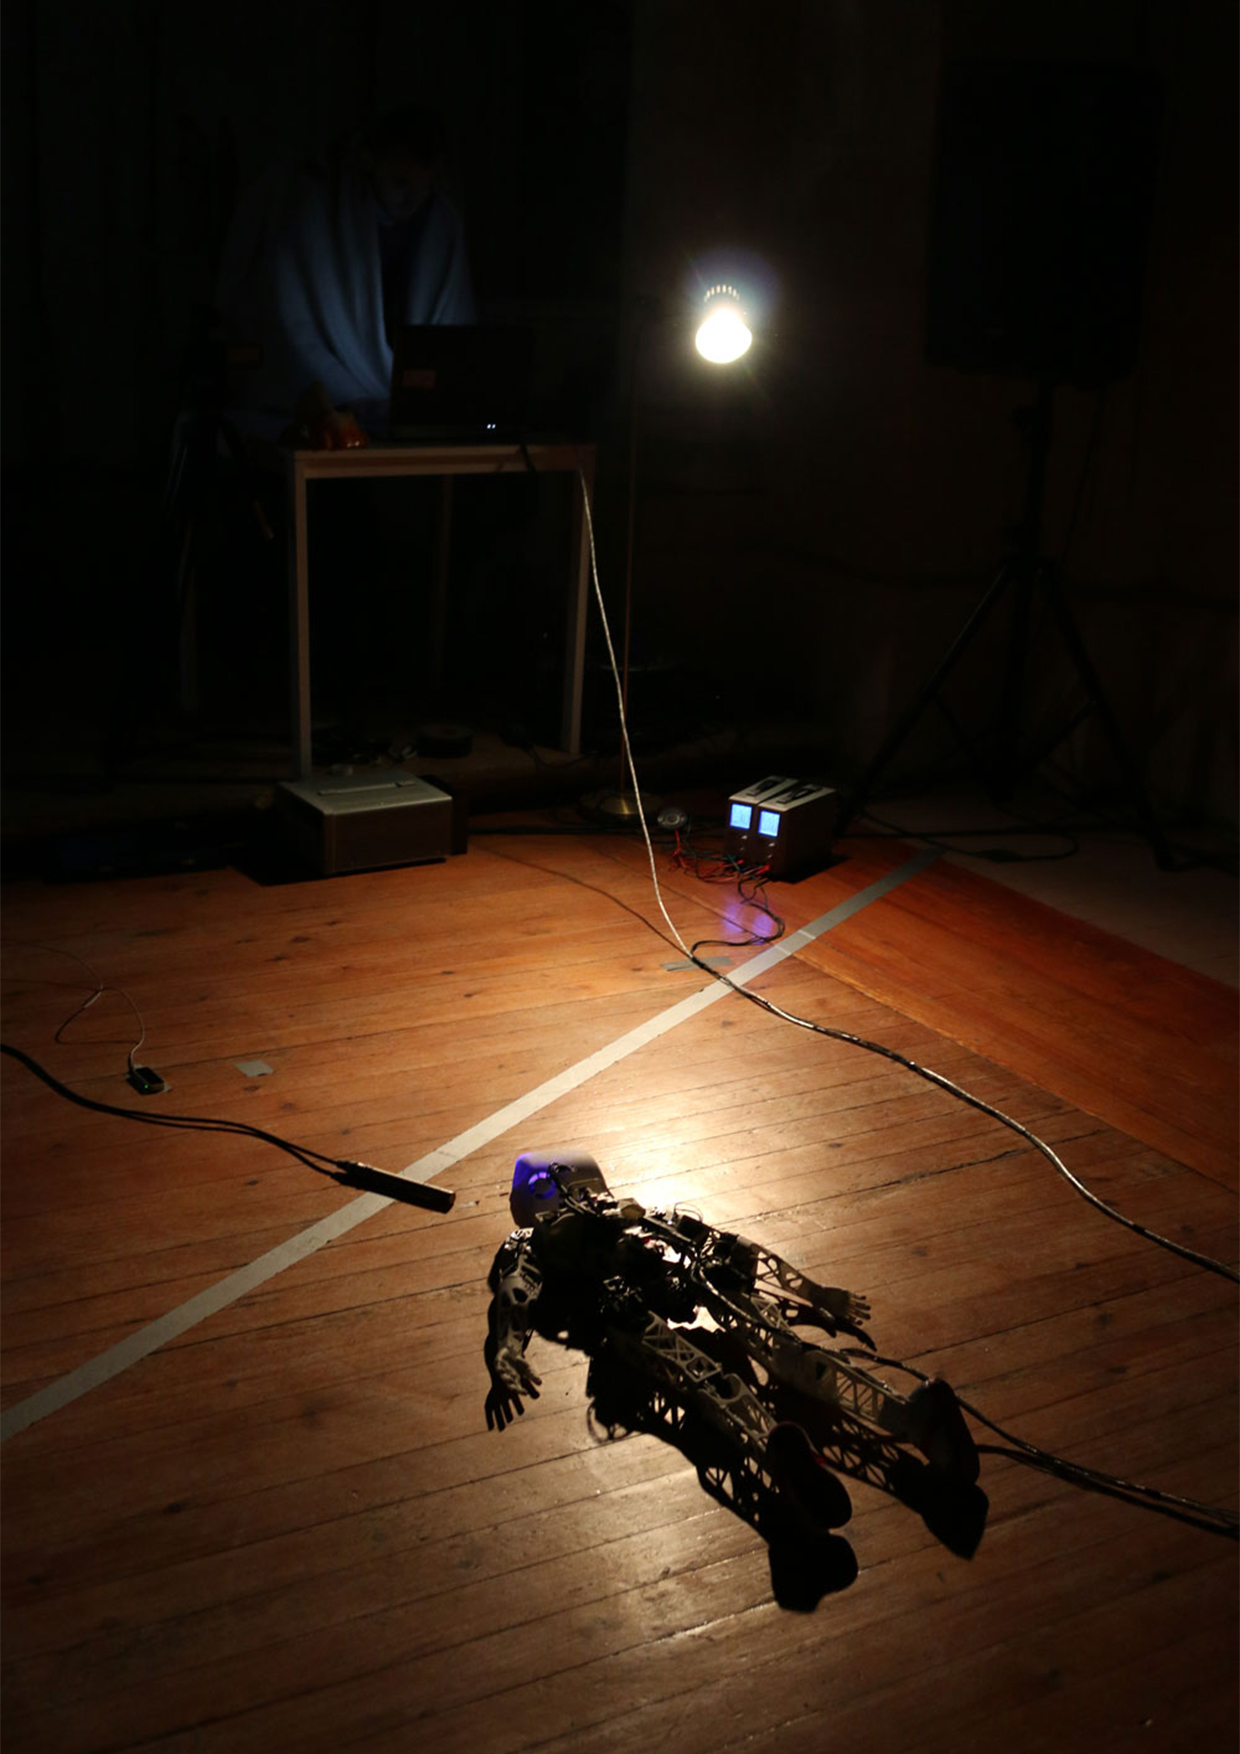
\includepdf{/Users/matthieulapeyre/Documents/phd_thesis/media/poppy_artist.pdf}

\chapter{The Poppy diffusion} % (fold)

\cleanchapterquote{Usage is like oxygen for ideas. You can never fully anticipate how an audience is going to react to something you’ve created until it’s out there. That means every moment you’re working on something without it being in the public it’s actually dying, deprived of the oxygen of the real world.}{Matt Mullenweg}

\section{The open source release} % (fold)

Poppy has been designed to go outside the lab

\subsection{Licenses} % (fold)

\subsection{The lack conversioning software for hardware} % (fold)

\section{Create a community} % (fold)

We created a community to share research, provide support and obtain contributions.
Sometimes, on technical aspects, hobbyist have more experience.

\subsection{Finding the good tools} % (fold)


\section{Pilot experiments} % (fold)

Poppy is an experimental tool design to be use outside the lab by 

Set up an open source release and community management tools are not enough. Our work needs to face the real world.

\subsection{LPPA} % (fold)

\subsection{\emph{Êtres et Numériques}: Arstist residency} % (fold)

\subsection{Universcience: hackathon} % (fold)

\subsection{Lycée Saintonge Sainte Famille} % (fold)

\subsection{ESAM} % (fold)




\section{Production/Distribution: an alternative approach} % (fold)

\subsection{A research lab is not a Start-Up} % (fold)
Poppy includes three main parts: its mechatronic structure (skeleton and motors); its electronics; its software.

Reproducing and rebuilding the mechatronic structure is easy: the open-source skeleton can be printed on personal 3D printers (or using online services for higher quality printing), and motors are bought off-the-shelf (motors are currently not open-source, but very standard). Obtaining and using the software is very easy: just download on the Poppy web site.

But the fabrication of electronics is challenging. It is not yet possible to produce electronics components at home, and many institutional users do not have the competence or motivation to do so. There are some kickstarter projects going on a way to facilitate the process, yet they are not ready and won't be ready until a couple of years.

The current classical approach to build and distribute this electronics boards is to raise funding allowing the manufacturing of hundreds of boards which can then be sold by a distribution company. But a french research institute like Inria is not a distributor,  is not even legally allowed to do.

Furthermore, even if one could buy or build easily all components, some users (e.g. artists) might want to obtain and use an already fully assembled Poppy robot. Thus, a structure capable of building and distributing the electronics, as well as the mechatronics and/or the robot fully assembled is needed.

Yet, the mission of a research team at Inria is to do research, and find ways to apply and transfer the results of this research, but not directly to produce and sell a commercial product. If a commercial product can emerge from our research, one way to exploit it is to create a start-up company which will set up a business plan around it, probably based on a production in Asia and then a worldwide distribution to research laboratories, universities and fablabs (see Figure \ref{fig:classic})

\begin{figure}[h]
    \begin{center}
        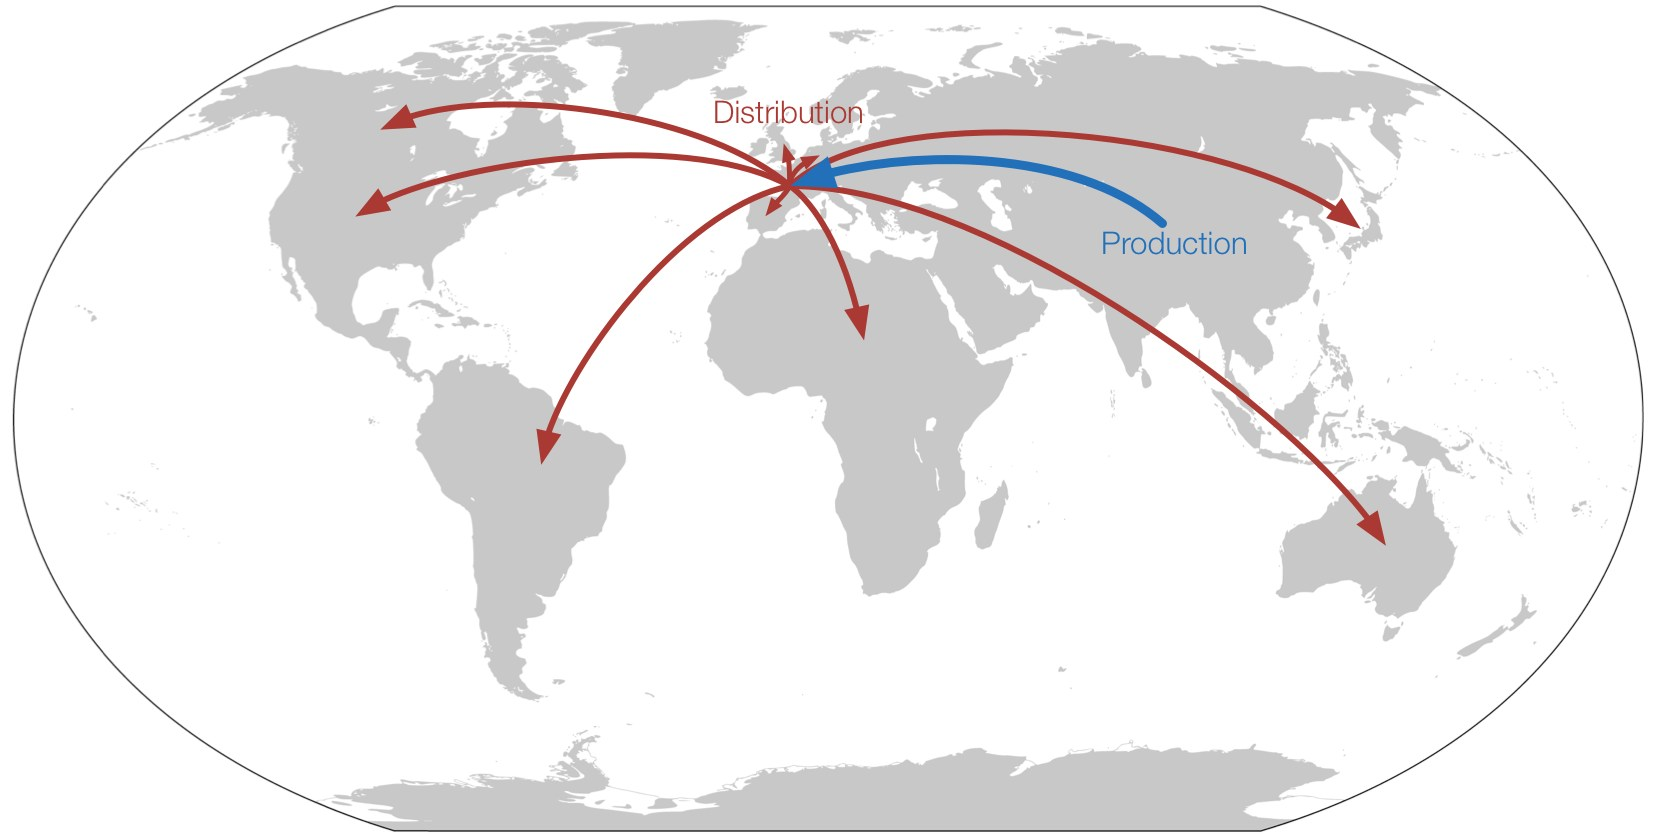
\includegraphics[width=14cm]{classic_production_distribution.jpg}
    \end{center}
    \caption{Classical approach for technology production and distribution}
    \label{fig:classic}
\end{figure}


But Poppy is not designed to be a standard commercial product. While it might foster the creation of an economical ecosystem and jobs, its main purpose is to become an educational tool that remains open, as well as rather low cost and easily reproducible. If the goal would have been to make it profitable, it would be necessary to sell it at a much higher price. The robot wouldn't be as accessible at it should to ensure the achievement of its scientific diffusion and educational missions... We would loose the intrinsic purpose of Poppy.

\section{Toward local open factories } % (fold)

Meanwhile, the "makers revolution" is gaining momentum (Chris Anderson) and more and more Fablabs are created around the world. As a main mission of Poppy is to be a educational platform, Poppy could become a popular platform used, hacked, transformed within the natural FabLab activities. But also, and this is the direction explored below,  it would make sense that  Poppy, as a whole or subsets of its components, be produced and distributed by Fablabs, and thus becoming a tool used by Fab Lab to develop and robustify the economic ecosystem in which they live.

\subsection{An alternative model } % (fold)

An original and constructive organizational process would be to take advantage of the production phase for educational purposes. In this context, each fablab would have the possibility to produce, assemble and sell Poppy to local actors (see Figure \ref{fig:word_fab}). Thus the production phase can become a training support for the use of 3D printing techniques and the manufacturing of electronic circuits, and later on be exploited through selling the constructed platforms.


\begin{figure}[tb]
    \begin{center}
        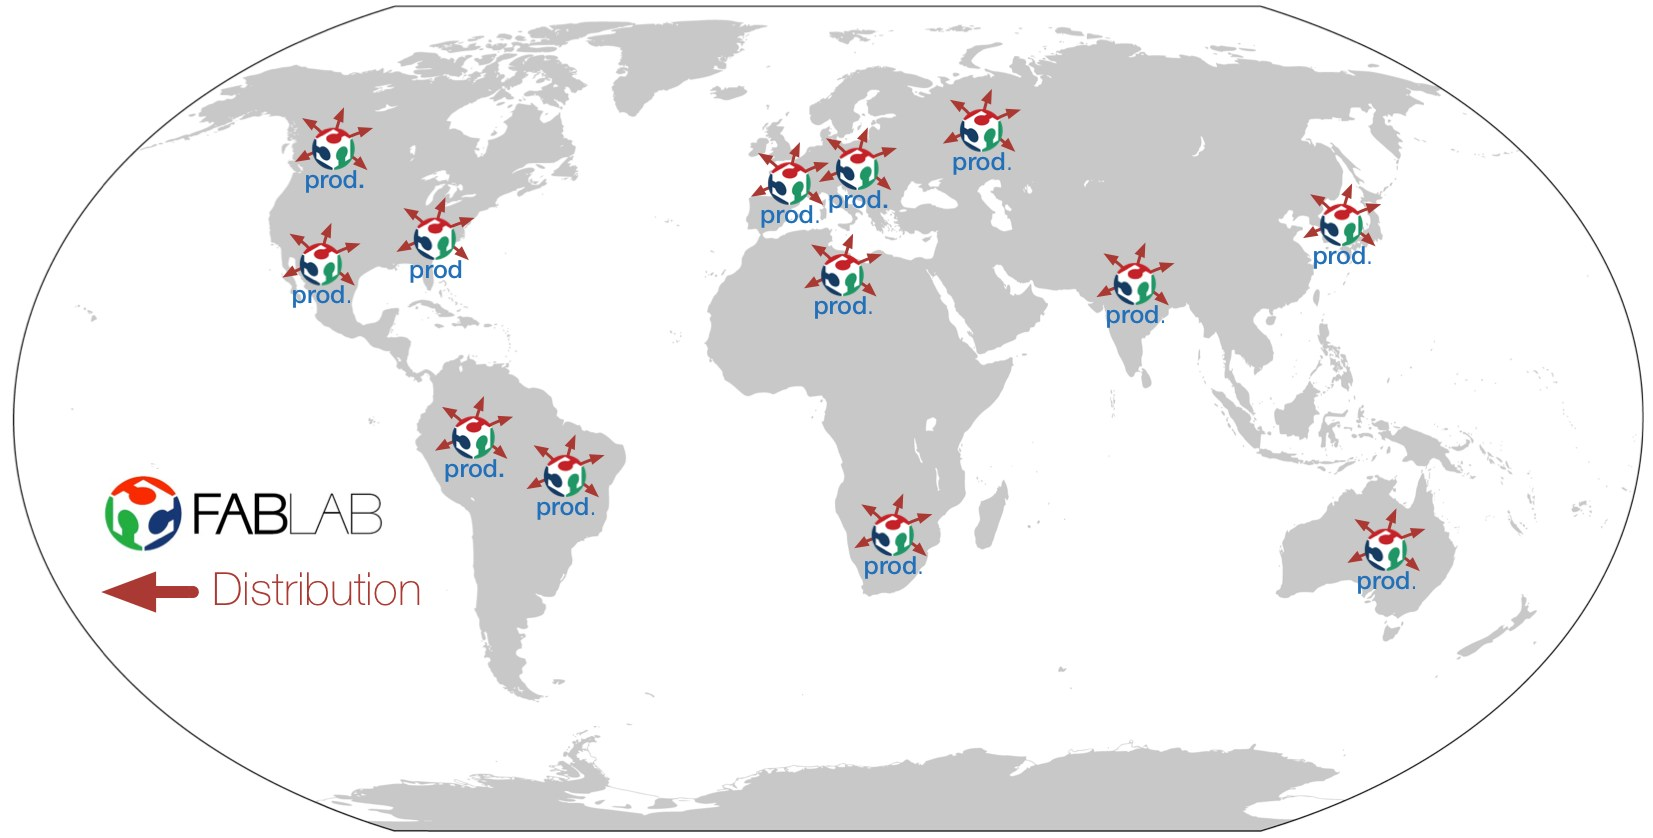
\includegraphics[width=14cm]{fabusine_distribution_world.jpg}
    \end{center}
    \caption{Fabrication and distribution locally done by Fablabs}
    \label{fig:word_fab}
\end{figure}


Also in a context where fablabs need to find an economic model, several sources of income may be found thanks to the distribution of platforms such as Poppy. The first and most obvious one is the sale to local actors of fully-assembled and functional Poppy robots produced by the Fablab. But a more advanced model can emerge. Poppy is a development robotic platform: it means that it can and will be broken, meaning that Fablabs may extend theirs commercial offers to:

\begin{itemize}
    \item Ensure a support (repairs, upgrades, ...) and may sell maintenance contracts with labs/school/university and even other 3rd party FabLabs.
    \item Provide a customisation service to adapt Poppy to specific needs (e.g. a university or lycée that would like to have a Poppy on wheels rather than legs)
    \item For an event or artist residency: The FabLab could rent a robot and provide a technician,
    \item Propose profesional formation to 3D printing to companies
    \item ...
\end{itemize}

From these kinds of interaction, links and collaboration between local actors and Fablabs may emerge leading to other potentially funded projects.

\subsection{Promote local collaboration } % (fold)

Beyond the act of production and sales, Poppy becomes a pretext to promote the linkage and exchange between local actors from multiple backgrounds. At the scale of a city or region, we can easily imagine a distribution of roles where several FabLabs could collaborate to build and distribute different parts of Poppy depending on their motivations, skills and equipements.
Also, it helps to connect the fablabs with local actors, public / private research labs, companies, schools/universities or artists (see Figure \ref{fig:local_synergy})

\begin{figure}[tb]
    \begin{center}
        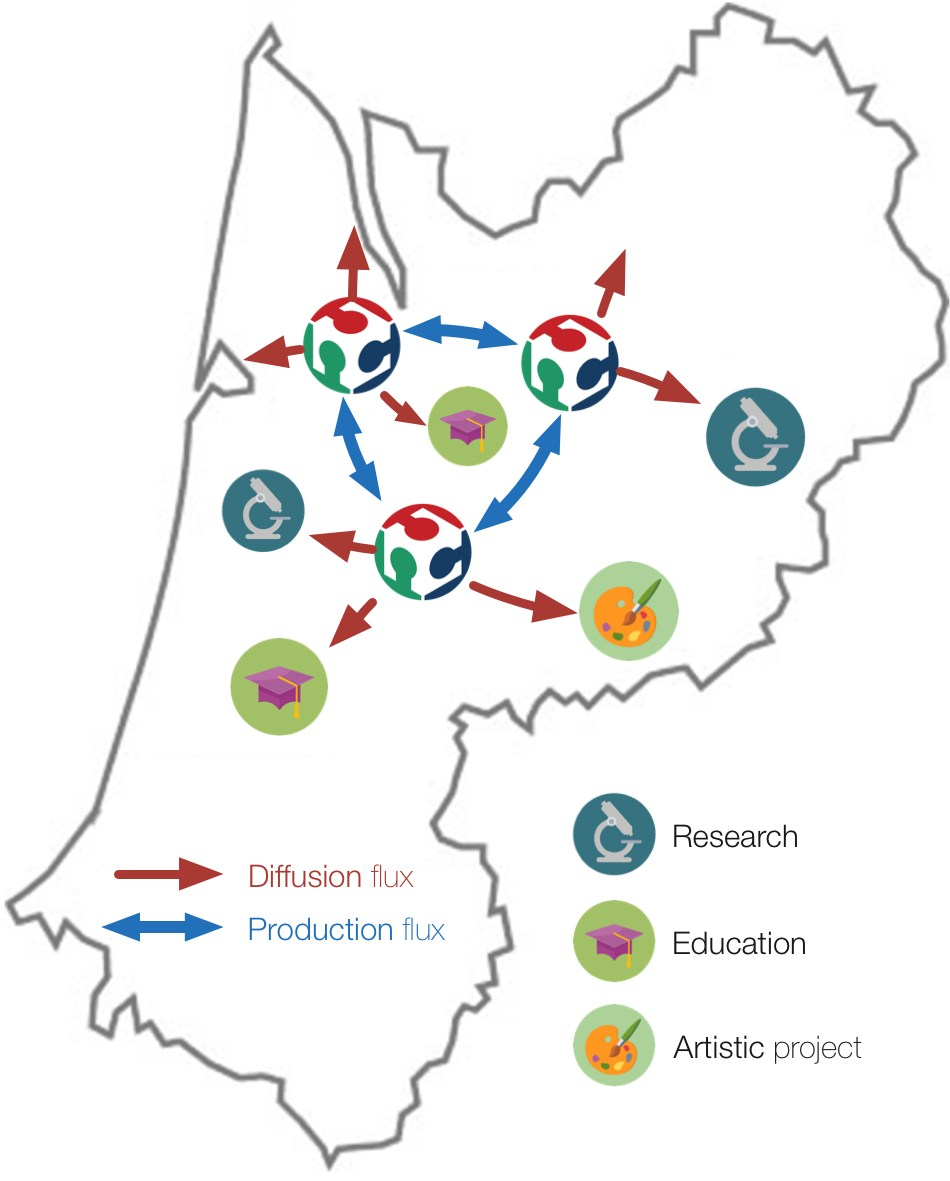
\includegraphics[height=10cm]{fabusine_local.jpg}
    \end{center}
    \caption{A synergy can emerge between Fablabs and local actors}
    \label{fig:local_synergy}
\end{figure}

\subsection{What is the role of the Flowers research team in such a process? } % (fold)

The Flowers research team's role remains essential. As the founders, designers and leaders of both the technological platform and its surrounding philosophy of openness and innovation, the Flowers team continues to improve the platform, take a central role in animating the community of users, and design new uses with scientists, educators, geeks and artists. Within this process, the Flowers team also coordinates the growing of the community of contributors and users, and designs strategies to ensure both the quality and sustainable development of the platform and its uses.

Among the tools used by the Flowers team to ensure such quality and sustainable development is through the control of the "Poppy" brand, and through policies/charters:

\begin{itemize}
\item The "Poppy" brand is owned by Inria, and the use of the brand by 3rd parties like FabLabs will only be possible through agreements ensuring that the Poppy project policies and philosophy is implemented;
\item Agreements take the form of charters/policies between Inria and FabLabs specifying guidelines to follow to ensure both quality and that each party (Inria, FabLab, users) finds its interest.
\end{itemize}

On the Inria side, the creation of an association which role would be to spin-off this technology development, community animation and quality control, is under consideration.






